
We analyze and quantify the improvement obtained by our rare word translation approach and provide a detailed 
comparison of the different rare word techniques proposed in Section~\ref{sec:rare}. We also examine the effect of 
depth on the LSTM architectures and demonstrate a strong correlation between perplexities and BLEU scores. We also highlight 
a few translation examples where our models succeed in correctly translating OOV words, and present 
several failures.

\subsection{Rare Word Analysis}
\begin{sloppypar}
To analyze the effect of rare words on translation quality, 
we follow Sutskever et al.~\cite{sutskever14} and sort sentences in 
newstest2014 by the average inverse frequency of their words. 
We split the test sentences into groups where the sentences within each group have a comparable number of rare words
 and evaluate each group independently. We evaluate our 
systems before and after translating the OOV words and compare with 
the standard MT systems -- we use the best system from the WMT'14 contest \cite{durrani-EtAl:2014:W14-33},
and neural MT systems -- we use the ensemble systems described in \cite{sutskever14} and Section~\ref{sec:exp}.
\end{sloppypar}

Rare word translation is challenging for neural machine translation systems as
shown in Figure~\ref{f:rare}. Specifically, the translation quality of our
model before applying the postprocessing step is shown by the green curve, and the current
best NMT system \cite{sutskever14} is the purple curve. While \cite{sutskever14}
produces better translations for sentences with frequent words (the left part of the
graph), they are worse than best system (red curve)
on sentences with many rare words (the right side of the graph). When applying our
unknown word translation technique (purple curve), we
significantly improve the translation quality of our NMT: 
for the last group of 500 sentences which have the greatest proportion of 
OOV words in the test set, we increase the BLEU score of our system by 
\imprare{} BLEU points. Overall, our rare word translation model 
interpolates between the SOTA system and the system
of \newcite{sutskever14},  which allows us to outperform the winning entry of WMT'14
on sentences that consist predominantly of frequent words and approach its performance on sentences
with many OOV words.
\begin{figure}
\centering
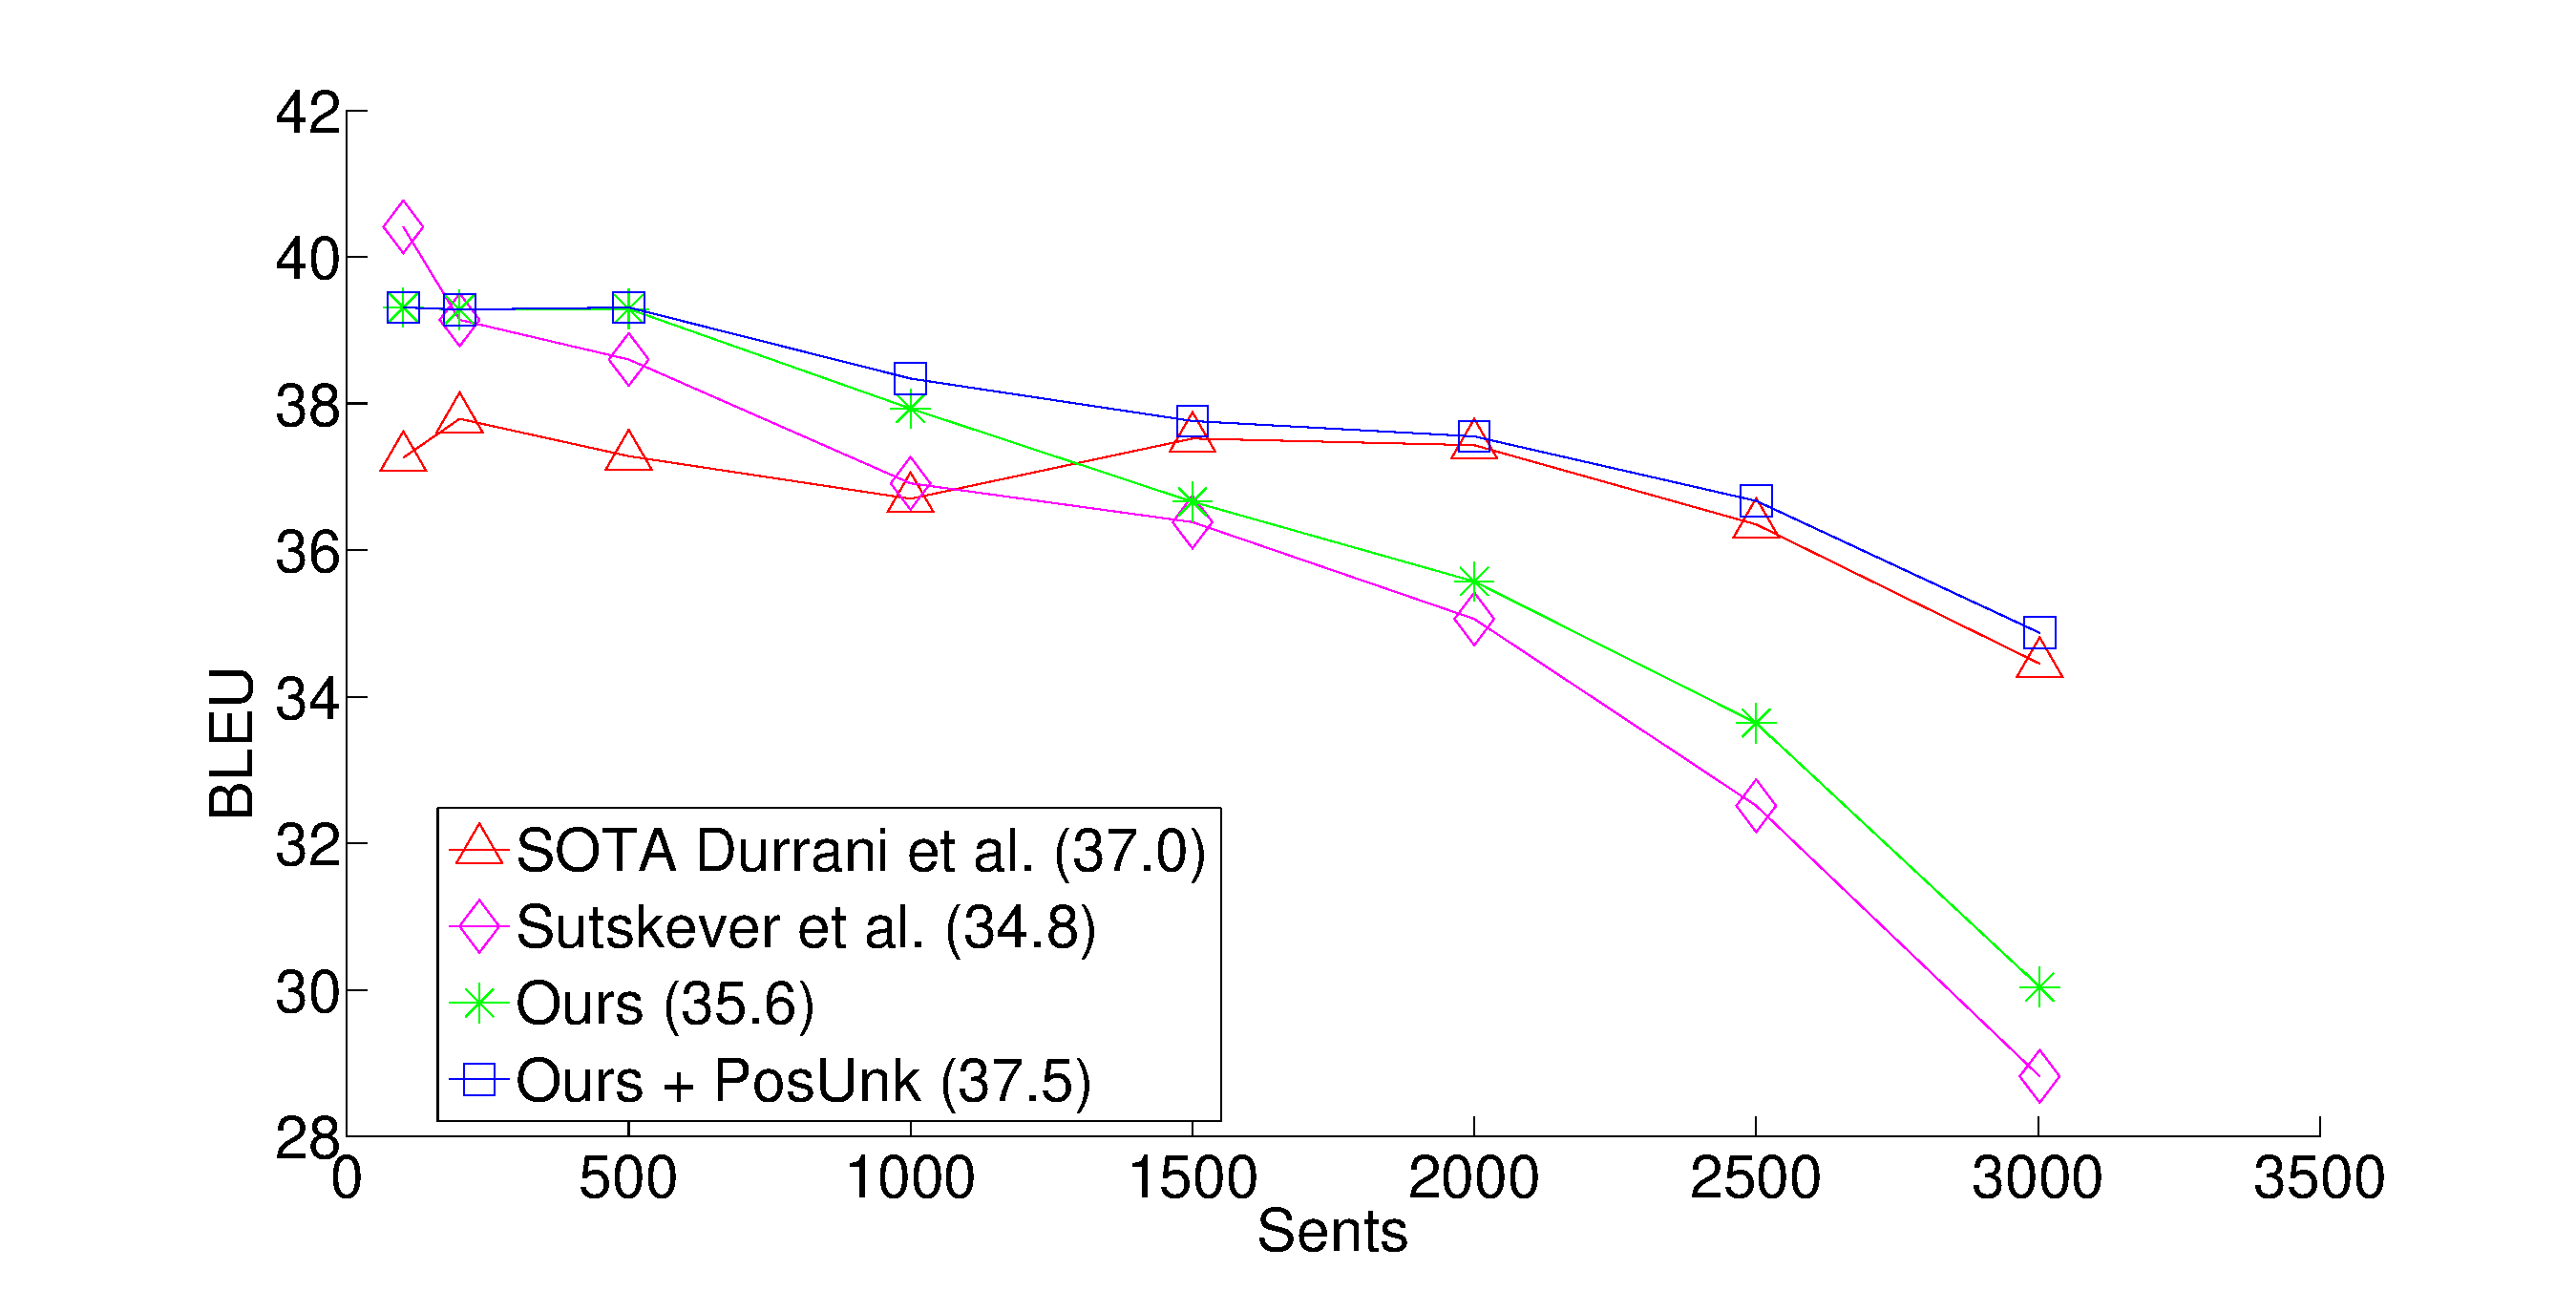
\includegraphics[width=0.7\textwidth, clip=true, trim= 95 0 230 0]{img/3-rare} % , angle=-90
\caption[Rare word translation]{{\bf Rare word translation} -- 
On the x-axis, we order newstest2014 sentences by their {\it average frequency rank} and divide the sentences into groups 
of sentences with a comparable prevalence of rare words. 
We compute the BLEU score of each group independently.} 
\label{f:rare}
\end{figure}


\subsection{Rare Word Models}
\label{subsec:rare_model_compare}

We examine the effect of the different rare word models presented in
Section~\ref{sec:rare}, namely: (a) {\it Copyable} -- which aligns the unknown
words on both the input and the target side by learning to copy indices, (b) the Positional All
({\it PosAll}) -- which predicts the aligned source positions for every target
word, and (c) the Positional Unknown ({\it PosUnk}) -- which predicts the aligned
source positions for only the unknown target words.\footnote{In this section and in section~\ref{subsec:effects},
all models are trained on the unreversed sentences, and we use the following hyperparameters: 
we initialize the parameters uniformly in [-0.1, 0.1], the learning rate is 1, the maximal gradient norm is 1, 
with a source vocabulary of 90k words, and a target vocabulary of 40k (see Section~\ref{subsec:train_details} for more details).
While these LSTMs do not achieve the best possible performance, it is still useful to analyze them.}
It is also interesting to measure the improvement obtained when no alignment information is used during training.
As such, we include a baseline model with no alignment knowledge ({\it NoAlign}) in which we simply assume that the $i^{\textrm{th}}$ unknown word on the target
sentence is aligned to the $i^{\textrm{th}}$ unknown word in the source sentence.

\begin{figure}
\centering
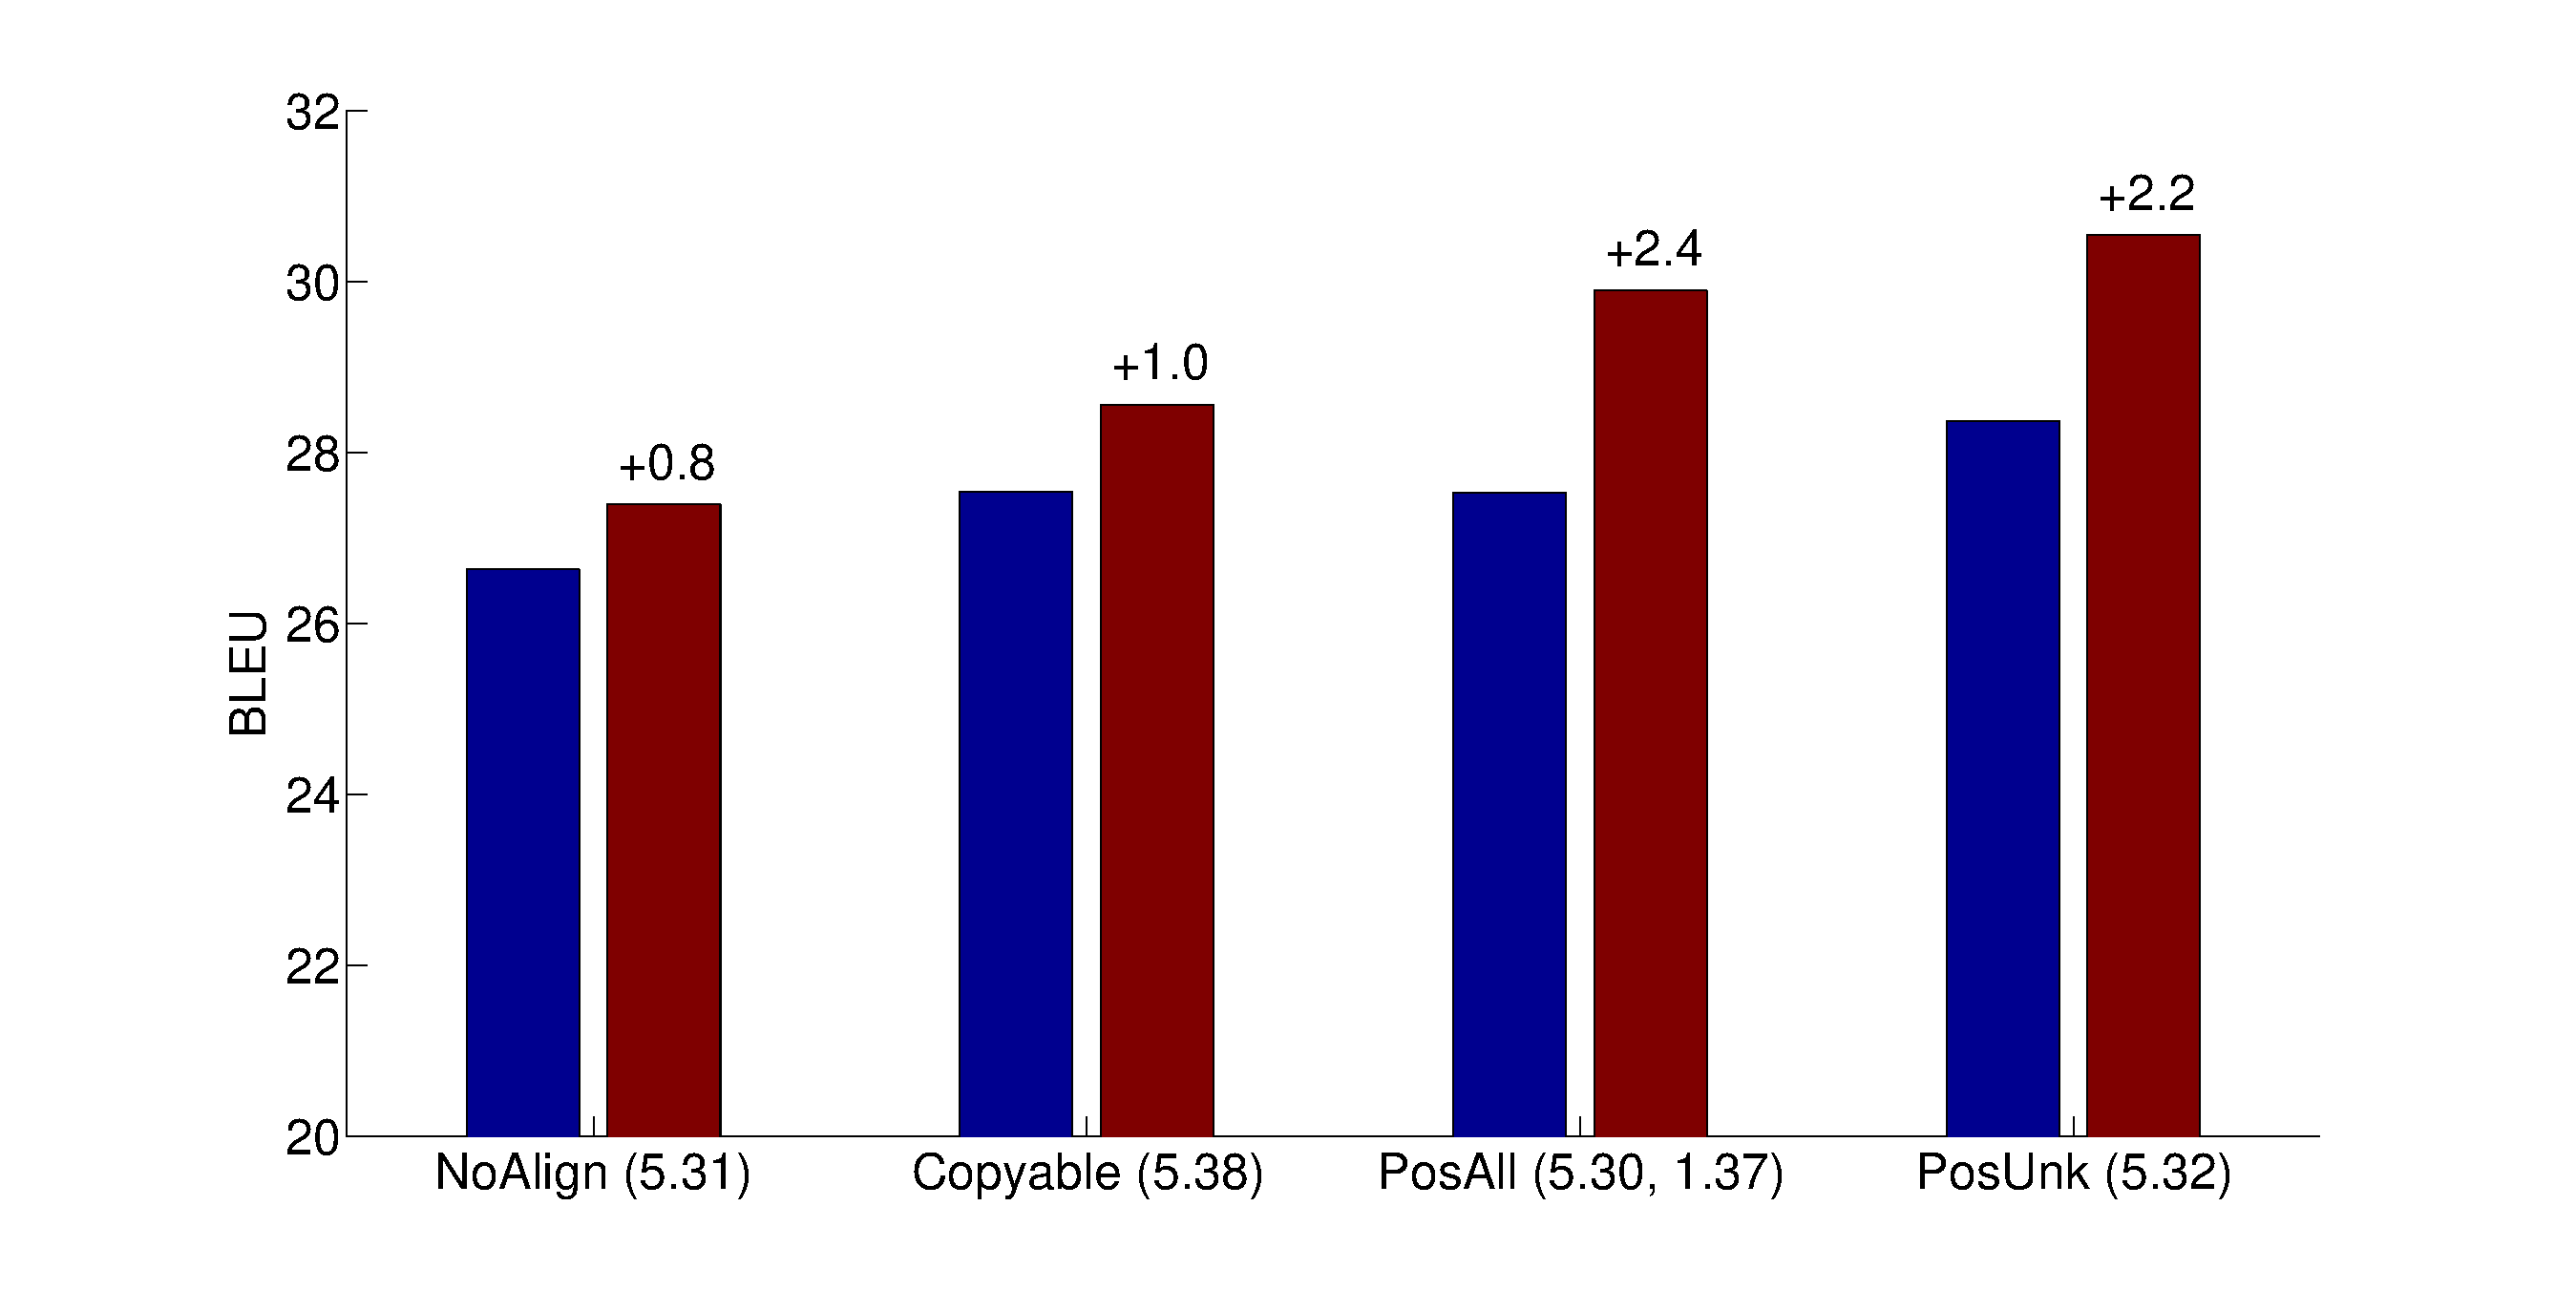
\includegraphics[width=0.7\textwidth, clip=true, trim= 105 0 140 0]{img/3-compare} % , angle=-90
\caption[Rare word models]{{\bf Rare word models} -- 
translation performance of 6-layer LSTMs:
a model that uses no alignment ({\it NoAlign}) 
and the other rare word models ({\it Copyable, PosAll, PosUnk}). 
For each model, we show results before ({\it left}) and after ({\it right}) the rare word translation as well as the perplexity (in parentheses).
For {\it PosAll}, we report the perplexities of predicting the words and the positions.} 
\label{f:compare}
\end{figure}

 
From the results in Figure~\ref{f:compare}, a simple monotone
alignment assumption for the {\it NoAlign} model yields a modest gain of
0.8 BLEU points. If we train the model to predict the alignment, then the {\it Copyable} model
offers a slightly better gain of 1.0 BLEU. Note, however, that English
and French have similar word order structure, so it would be
interesting to experiment with other language pairs, such as English and
Chinese, in which the word order is not as monotonic. These harder language pairs 
potentially imply a smaller gain for the NoAlign model and a larger
gain for the Copyable model. 
We leave it for future work.

The positional models ({\it PosAll} and {\it PosUnk}) 
improve translation performance by more than 2 BLEU points. 
This proves that the limitation of the copyable model, which forces
it to align each unknown output word with an unknown input word, is considerable.  
In contrast, the positional models can align the unknown target words with any source word,
and as a result, post-processing has a much stronger effect. 
The PosUnk model achieves better translation results than
the PosAll model which suggests that it is easier to train the LSTM on shorter sequences. 

\subsection{Other Effects}
\label{subsec:effects}
{\bf Deep LSTM architecture} --  We compare PosUnk models trained with different number of layers (3, 4, and 6). 
We observe that the gain obtained by the PosUnk model increases in tandem with the overall accuracy of the model, which is consistent 
with the idea that larger models can point to the appropriate source word more accurately.
Additionally, we observe that on average, each extra LSTM layer provides roughly 1.0 BLEU point improvement as demonstrated in Figure~\ref{f:depth}. 

\begin{figure}[tbh!]
\centering
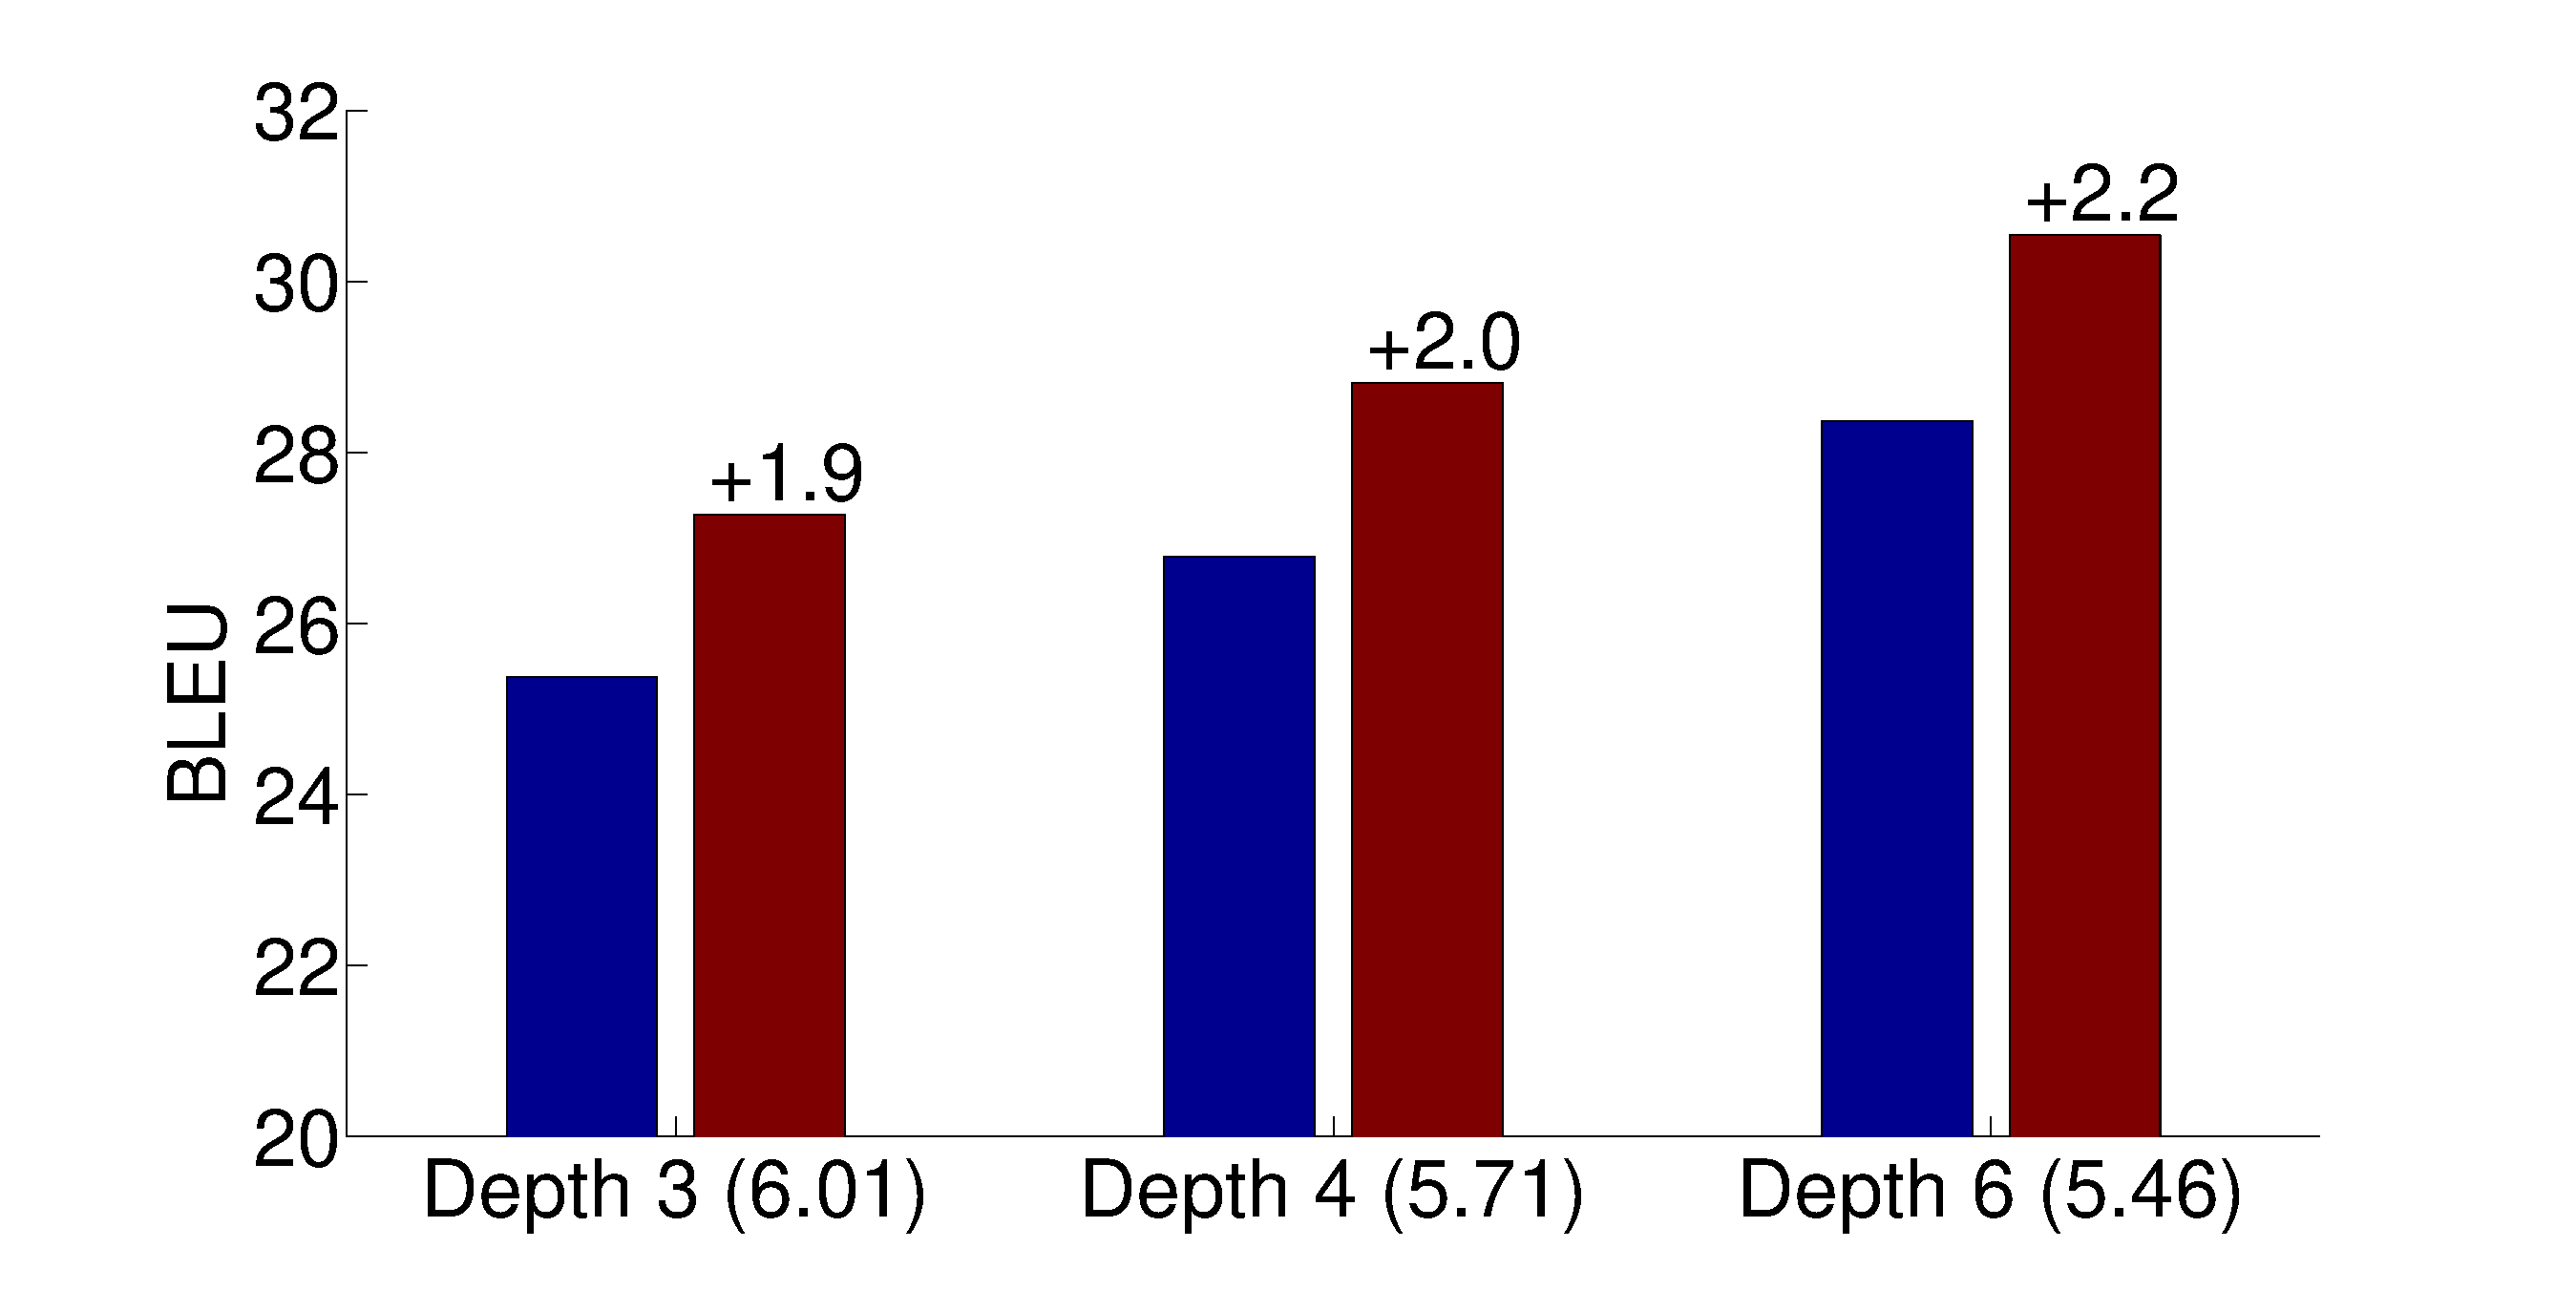
\includegraphics[width=0.7\textwidth, clip=true, trim= 0 0 0 0]{img/3-depth} % , angle=-90
\caption[Effect of depths]{{\bf Effect of depths} -- BLEU scores achieved by {\it PosUnk} models of various depths (3, 4, and 6) before and after the rare word translation. 
 Notice that the PosUnk model is more useful on more accurate models. }
\label{f:depth}
\end{figure}

{\bf Perplexity and BLEU} -- Lastly, we find it interesting to observe a strong correlation 
between the perplexity (our training objective) and the translation quality as measured by BLEU. 
Figure~\ref{f:cor} shows the performance of a 4-layer LSTM, in which we compute both perplexity and 
BLEU scores at different points during training. We find that on average, a reduction of 0.5 perplexity 
gives us roughly 1.0 BLEU point improvement.
\begin{figure}[tbh!]
\centering
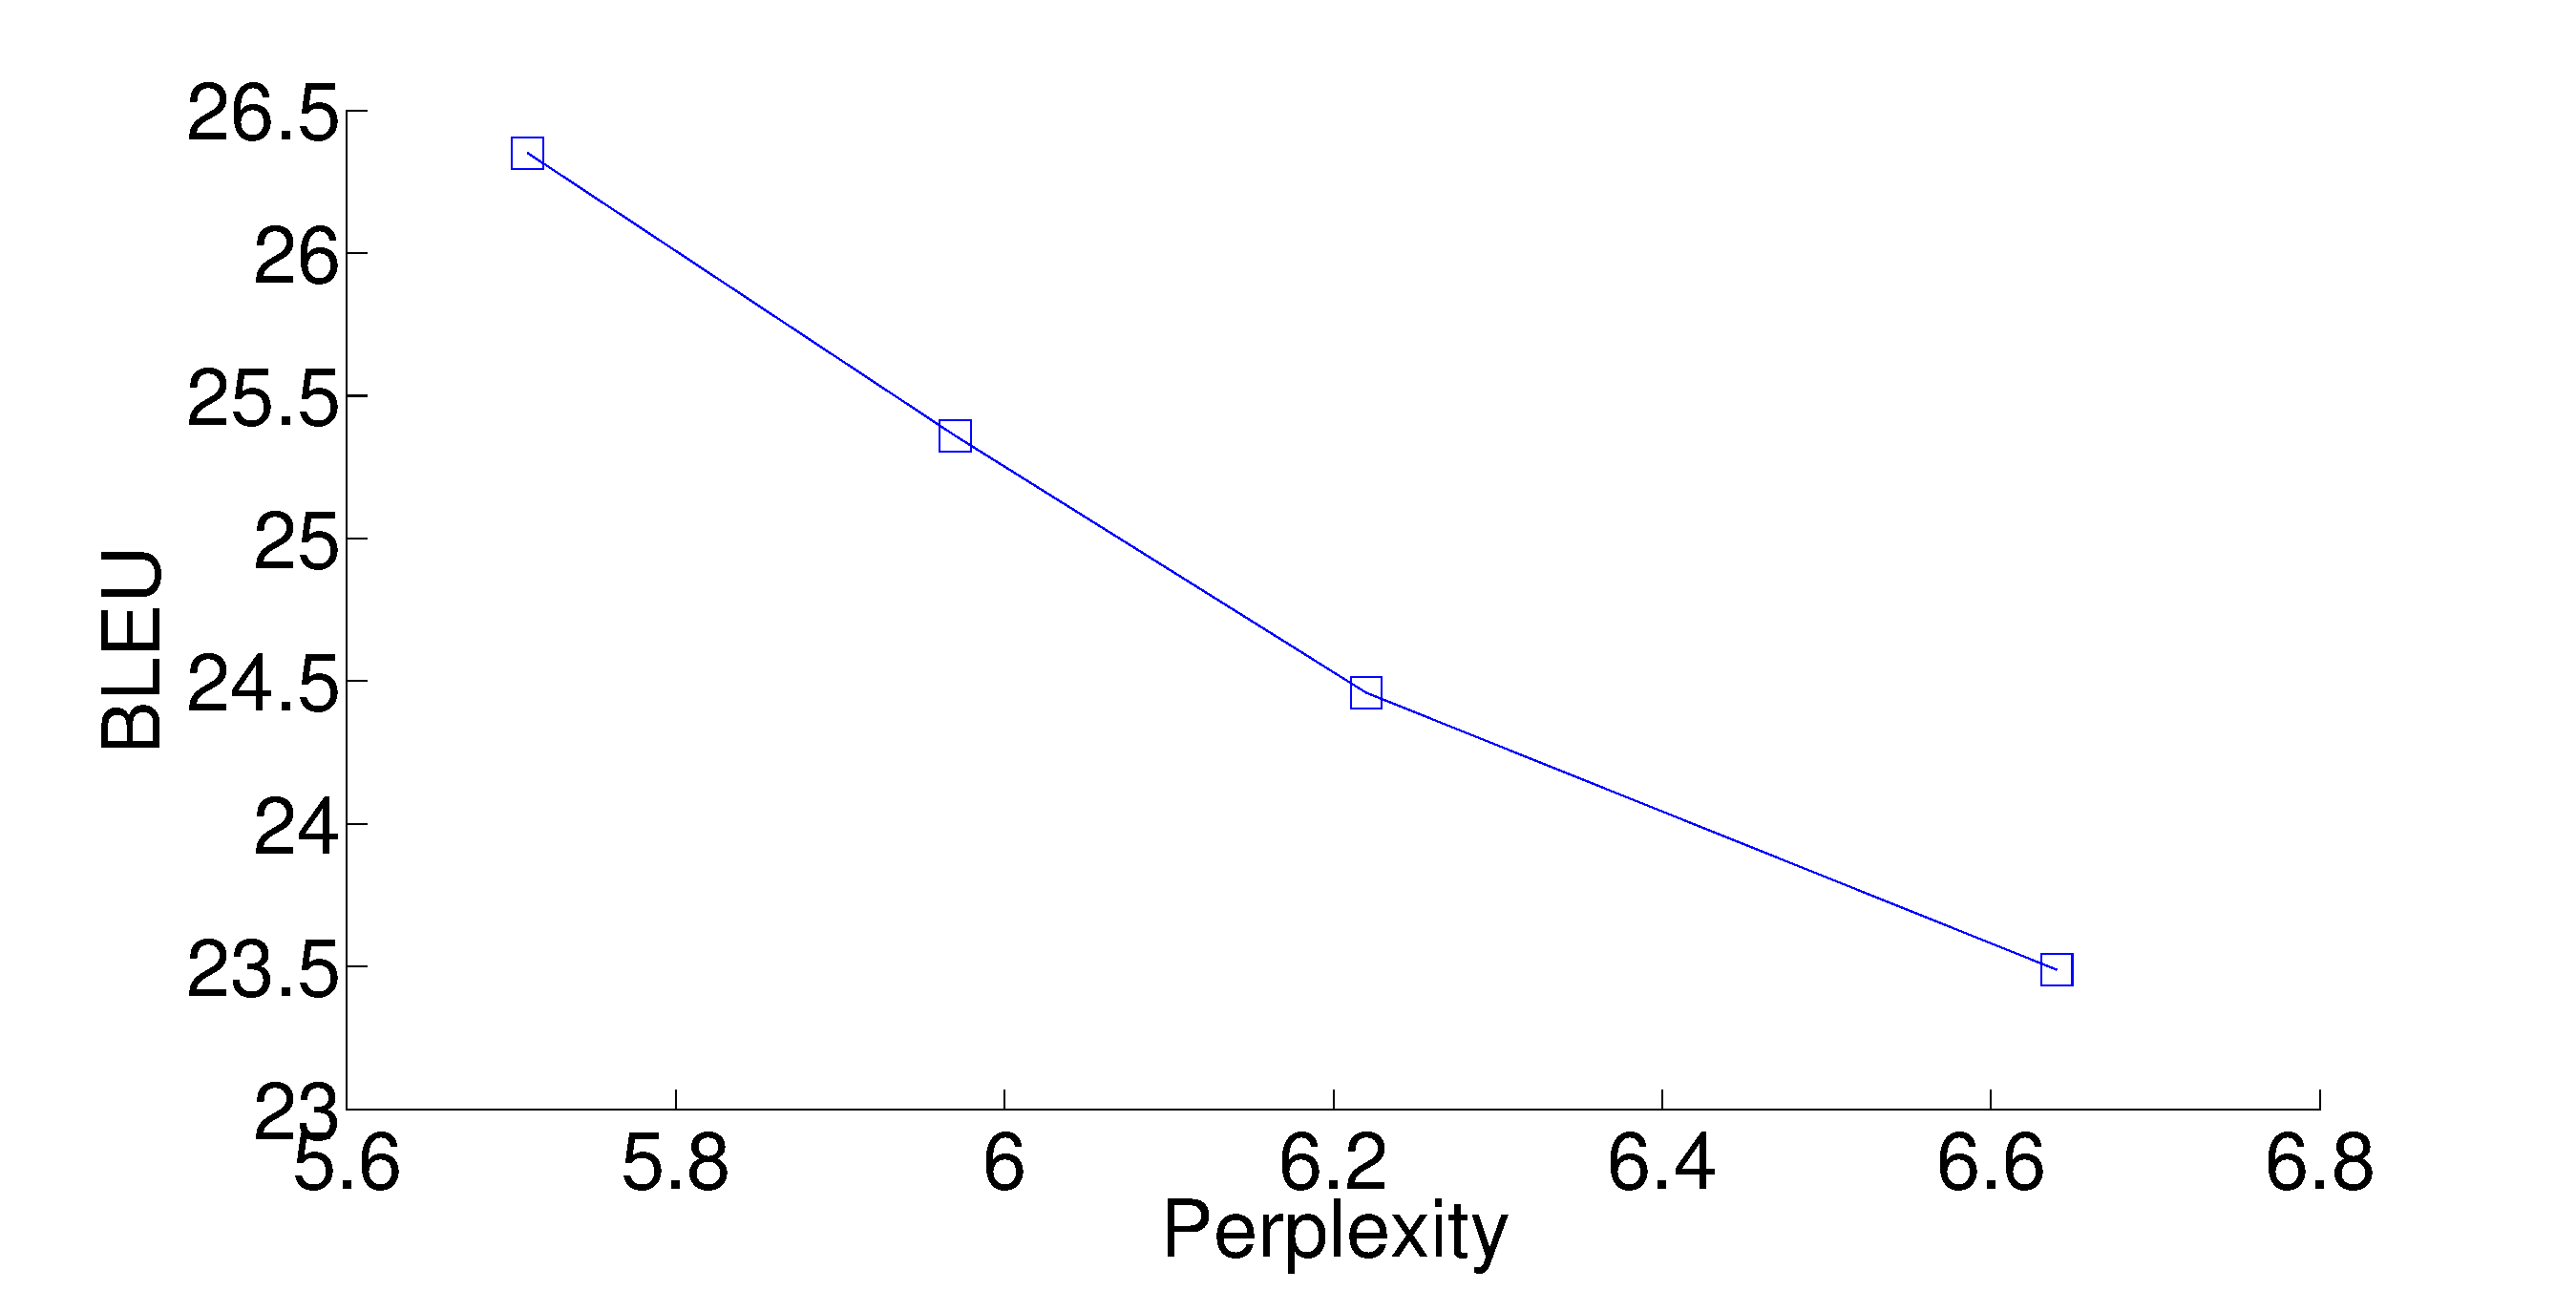
\includegraphics[width=0.7\textwidth, clip=true, trim= 0 0 0 0]{img/3-cor} % , angle=-90
\caption[Perplexity vs. BLEU]{{\bf Perplexity vs. BLEU} -- we show the correlation by evaluating an LSTM model with 4 layers at various stages of training. 
} 
\label{f:cor}
\end{figure}


\subsection{Sample Translations}
We present three sample translations of our best system
(with \bestbleuunk{} BLEU) in Table~\ref{t:sample}. In our  first example,
the model translates all the
unknown words correctly: {\it 2600}, {\it orthop{\'e}diques}, and {\it
cataracte}. It is interesting to observe that the model can accurately predict
an alignment of distances of 5 and 6 words. The second
example highlights the fact that our model can translate long
sentences reasonably well and that it was able to
correctly translate the unknown word for {\it JPMorgan} at the very far end of
the source sentence. Lastly, our examples also reveal several
penalties incurred by our model: (a) incorrect entries in the word dictionary, as with {\it n\'{e}gociateur} vs. {\it trader} in the second example, 
%identical meaning with different words, as with {\it n\'{e}gociateur} vs. {\it trader} in the second example, 
and (b) incorrect alignment prediction, such as when 
 \unkpostext{3} is incorrectly aligned
with the source word {\it was} and not with {\it abandoning}, which resulted in an
incorrect translation in the third sentence.

\begin{table*}[tbh!]
\centering
\resizebox{13.5cm}{!}{
\begin{tabular}{c|p{12cm}}
\bf{} & \bf{Sentences}\\
  \hline
src & An additional {\it 2600} operations including {\it orthopedic} and {\it cataract} surgery will help clear a backlog .\\
  \hline
trans & En outre , \unkpos{1} op{\'e}rations suppl{\'e}mentaires , dont la chirurgie \unkpos{5} et la \unkpos{6} , permettront de r{\'e}sorber l' arri{\'e}r{\'e} .\\
  \hline
+unk & En outre , {\it 2600} op{\'e}rations suppl{\'e}mentaires , dont la chirurgie {\it orthop{\'e}diques} et la {\it cataracte} , permettront de r{\'e}sorber l' arri{\'e}r{\'e} .\\
  \hline
tgt & 2600 op{\'e}rations suppl{\'e}mentaires , notamment dans le domaine de la chirurgie orthop{\'e}dique et de la cataracte , aideront {\`a} rattraper le retard .\\
  \hline
  \hline
src & This {\it trader} , Richard {\it Usher} , left RBS in {\it 2010} and is understand to have be given leave from his current position as European head of forex spot trading at {\it JPMorgan} .\\
  \hline
trans & Ce \unkpos{0} , Richard \unkpos{0} , a quitt{\'e} \unkpos{1} en 2010 et a compris qu' il est autoris{\'e} {\`a} quitter son poste actuel en tant que leader europ{\'e}en du march{\'e} des points de vente au \unkpos{5} .\\
  \hline
+unk & Ce {\it n\'{e}gociateur} , Richard {\it Usher} , a quitt{\'e} RBS en {\it 2010} et a compris qu' il est autoris{\'e} {\`a} quitter son poste actuel en tant que leader europ{\'e}en du march{\'e} des points de vente au {\it JPMorgan} .\\
  \hline
tgt & Ce trader , Richard Usher , a quitt{\'e} RBS en 2010 et aurait {\'e}t{\'e} mis suspendu de son poste de responsable europ{\'e}en du trading au comptant pour les devises chez JPMorgan \\
  \hline
  \hline
src & But concerns have grown after Mr {\it Mazanga} was quoted as saying {\it Renamo} {\it was} abandoning the 1992 peace accord .\\
  \hline
trans & Mais les inqui{\'e}tudes se sont accrues apr{\`e}s que M. \unkpos{3} a d{\'e}clar{\'e} que la \unkpos{3} \unkpos{3} l' accord de paix de 1992 .\\
  \hline
+unk & Mais les inqui{\'e}tudes se sont accrues apr{\`e}s que M. {\it Mazanga} a d{\'e}clar{\'e} que la {\it Renamo} {\it {\'e}tait} l' accord de paix de 1992 .\\
  \hline
tgt & Mais l' inqui{\'e}tude a grandi apr{\`e}s que M. Mazanga a d{\'e}clar{\'e} que la Renamo abandonnait l' accord de paix de 1992 .\\
\end{tabular}
}
\caption[Sample translations]{{\bf Sample translations} -- the table shows the source ({\it src}) and the translations of our best model before ({\it trans}) and after ({\it +unk}) unknown word translations. We also show the human translations ({\it tgt}) and italicize words that are involved in the unknown word translation process.}
\label{t:sample}
\end{table*}


